\chapter{Methodology}
In this chapter, each step that we followed in our method will be explained in detail.
\section{Structural Variation Discovery with HTS Data}
Structural variations are believed to be highly associated with diseases \cite{fanciulli2007fcgr3b,fellermann2006chromosome,aitman2006copy,gonzalez2005influence}. Therefore their discovery will be of critical importance in reducing the genetic disease susceptibility. Despite their significance in understanding disease susceptibility, there is no algorithm yet to find all types and sizes of structural variations at once. Before high-throughput sequencing technologies, microarrays were mainly used in structural variation discovery especially for copy number variation \cite{alkan2011genome}. As reviewed by Alkan et al., microarrays are no good at discovering balanced rearranagements and also are not able to locate the copy number variations \cite{alkan2011genome}. 

Although some are originally designed for old sequencing technologies, high-throughput sequencing platforms have brought novel methods for structural variation discovery. 
\subsection{Read Pair}
Paired-end sequencing is a sequencing method where reads are generated from both sides of a DNA fragment whose distance known. The distance information will be used later by the aligner while aligning the paired-end reads to the reference genome. Read pair method utilizes the distance information between paired-end reads \cite{tuzun2005fine}. As shown in the Figure \ref{readpair}, paired-end reads that align too distant from each other indicates a deletion, those align too close to each other indicates an insertion.

\begin{figure}[ht]
    \centering
    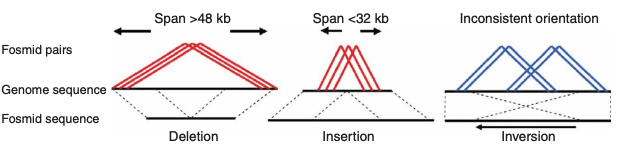
\includegraphics[scale=0.4]{images/readpair.png}
    \caption{(adapted from \cite{tuzun2005fine})}
    \label{readpair}
\end{figure}
\subsection{Read Depth}
Read depth is a simple method to detect duplications and deletions at a higher resolution. Based on the assumption that regions are randomly sequenced, for reads that are mapped to all possible locations of the reference genome, the depth of duplicated regions will be higher and the depth of deleted regions will be lower than average \cite{bailey2002recent} as shown in Figure \ref{readdepth}. Multiple read-mapping is an important aspect of read depth to work effectively. Otherwise the diffence of depth between duplicated regions and deleted regions will be insignificant. However known sequencing bias against GC-rich and GC-poor regions \cite{smith2008rapid} should be handled carefully.

\begin{figure}[ht]
    \centering
    
\includegraphics[scale=0.4]{images/placeholder.jpg}
    \caption{Read depth figure will be added}
    \label{readdepth}
\end{figure}

\subsection{Split Read}
Originally designed for longer reads (Sanger sequence etc.), split read based methods were capable of structural variation discovery at one base pair resolution by trying to map the reads by splitting. Similar to read pair, the location of split reads will tell the class of structural variation. For instance, the distance between split reads shows an insertion or first split coming after second split indicates an inversion.

\subsection{Sequence Assembly}
Although it is in its early stages, sequence assembly methods are, in theory, powerful and requires less computational power. Assuming the whole genome is assembled without using the reference genome (\textit{de novo} assembly), we can easily detect structural variation by comparing the individual's genome with the reference genome.

\section{Data Preprocessing}
We have the data showing the genome-wide segmental duplications (SD). The data consist of SD pairs with their exact locations. Furthermore, we have global alignments of SD pairs in a file generated using ClustalW \cite{thompson1994clustal}. Since entries in our data show the duplications in pairs, we had to identify SD groups in order to locate singly unique nucleotide positions. 

\begin{algorithm}
\caption{Missing Pairs}\label{missingPairs}
\begin{algorithmic}[1]
\Procedure{Find\_Missing\_Pairs}{}
\State $\textit{M} \gets \text{map of }\textit{Segmental Duplications}\text{ as read from data}$
\For{$\text{each key-value pair in }\textit{M}$}
\For{$\text{value}$}
\State $\textit{temp\_set} \gets \text{M{[value]}}$
\State $\text{clear M{[value]}}$
\EndFor
\While{true}
\State $\textit{flag} \gets \text{true}$
\For{$\text{each key-value pair in }\textit{M}$}
\State $\textit{Find intersection of }\textit{temp\_set}\text{ and }\textit{value}$
\If{$\text{intersection is not empty}$}
\State $\textit{flag} \gets \text{false}$
\State $\textit{temp_set} \gets \textit{value}$
\EndIf
\EndFor
\EndWhile
\EndFor
\EndProcedure
\end{algorithmic}
\end{algorithm}

\section{Extracting Singly Unique Nucleotides}
\subsection{Singly Unique Nucleotides (SUN)}
\section{Depth of Coverage}
\subsection{GC Correction}
